\documentclass[../paper.tex]{subfiles}

% Document
\begin{document}
    GraphCast is a machine learning-based method developed by Google DeepMind for medium-range global weather forecasting.
    It is an autoregressive model based on graph neural networks and a novel high-resolution multiscale mesh representation.
    It is a mesh representation that is used to represent the Earth's surface and atmosphere.
    The mesh is a grid of points that are connected by lines to form triangles.
    The mesh is multiscale, meaning that it has different resolutions at different levels.
    The mesh is high-resolution, meaning that it has a high density of points, which allows for more accurate predictions.
    GraphCast is trained on historical weather data from the European Centre for Medium-Range Weather Forecasts (ECMWF)'s ERA5 reanalysis archive\cite{e1}.
    \\\\
    It starts with the current state of Earth's weather and data about the weather six hours ago.
    Then, it makes a prediction about what the weather will look like six hours from now.\\
    GraphCast then feeds those predictions back into the model, performs the same calculation, and spits out longer-term forecasts\cite{e1}.\\
    \begin{figure}[htbp]
        \centerline{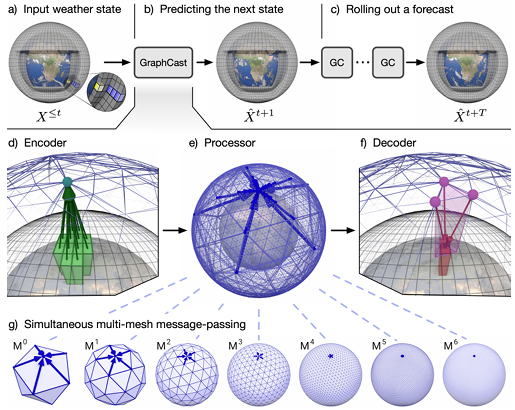
\includegraphics[width=0.4\textwidth]{../photos/multimesh_graphcast}}
        \caption{Steps of GraphCast}
        \label{fig:multimesh-graphcast}
    \end{figure}\\
    GraphCast's multiscale mesh representation. \\
    a) First, we insert the data into the model.
    b) Then we perform GraphCast to predict data, we feed this data back into the model.
    c) We perform GraphCast again to predict data, we feed this data back into the model and do this repeatedly.
    d) The encoder component maps local regions of the input (the green boxes) into nodes of the multi-mesh graph representation.
    e) The processor component performs a series of graph neural network (GNN) message passing steps to update the node features.
    f) The decoder component maps the updated node features back to the output (the purple boxes).
    g) The multi-mesh is a set of icosahedral meshes of increasing resolution, from the base mesh ($M^0$, 12 nodes) to the finest resolution ($M^6$ , 40, 962 nodes), which has uniform resolution across the globe.
    Each node belongs to a particular mesh resolution, and is connected to all neighboring nodes at the same resolution, as well as higher resolutions.
    The learned message-passing over the different meshes' edges happens simultaneously, so that each node is updated by all of its incoming edges.
    \\\\
    The package contains example code to run and train GraphCast.
    It also provides three pretrained models: GraphCast, the high-resolution model used in the GraphCast paper (0.25 degree resolution, 37 pressure levels),
    trained on ERA5 data from 1979 to 2017, Grap\_Cast\_small, a smaller, low-resolution version of GraphCast (1 degree resolution,
    13 pressure levels, and a smaller mesh), trained on ERA5 data from 1979 to 2015, useful to run a model with lower memory and compute constraints,
    GraphCast\_operational, a high-resolution model (0.25 degree resolution, 13 pressure levels) pretrained on ERA5 data from 1979 to 2017
    and fine-tuned on HRES data from 2016 to 2021\cite{e2}.

    \subsubsection{Advantages}
    Here are some of the advantages of GraphCast:
    \begin{itemize}
        \item \textbf{Accuracy} - GraphCast outperforms the most accurate previous ML-based weather forecasting model on percent 99.2 of the 252 targets it reported on\cite{e1}.
        \item \textbf{Speed} - GraphCast can generate a 10-day forecast (35 gigabytes of data) in under 60 seconds on Cloud TPU v4 hardware\cite{e1}.
    \end{itemize}

    \subsubsection{Disadvantages}
    Despite the advancement, GraphCast has limitations. \\
    \begin{itemize}
        \item \textbf{Accuracy} - GraphCast is not yet able to predict extreme weather events, such as hurricanes, tornadoes, and floods.
        At least not accurately.
        It did not outperform conventional models in all scenarios, such as the sudden intensification of Hurricane Otis, which hit Acapulco with minimal warning on October 25, 2023\cite{e4}.
        \item \textbf{Transparency} - GraphCast is a black box model, meaning that it is not possible or hard to understand how it works.
    \end{itemize}

    \subsubsection{Motivation}
    GraphCast is a fast and accurate weather forecasting model, that outperforms conventional models in most scenarios.\\
    It also provides pretrained models, which makes it easier to implement in our application.
    No need to train our own model.
    \\\\
    It also makes use of the ECMWF's ERA5 reanalysis archive, which is the same data source that OpenWeatherMap uses.
    It is known to be accurate.


\end{document}